\documentclass[tikz,border=0pt]{standalone}
\usepackage[T1]{fontenc}
\usepackage[utf8]{inputenc}
\usepackage{amsmath,amssymb}

%% ACM
\usepackage[tt=false, type1=true]{libertine}
\usepackage[varqu]{zi4}
\usepackage[libertine]{newtxmath}

%% IEEE
%\renewcommand{\sfdefault}{phv}
%\renewcommand{\rmdefault}{ppl}
%\renewcommand{\ttdefault}{pcr}
%\usepackage{mathptmx}

\usepackage{pgfplots}
\pgfplotsset{compat=1.18}
\usepgfplotslibrary{groupplots}
\usepgfplotslibrary{colormaps}
\tikzset{
	bar-color/.style={
		color of colormap={#1},
		draw=.!80!black,
		fill=.!80!white,
	},
	normal-color/.style={
		color of colormap={#1},
		draw=.,
	},
	mydashed/.style={dash pattern=on 6pt off 4pt}
}

\begin{document}

% This file was created by tikzplotlib v0.9.8.
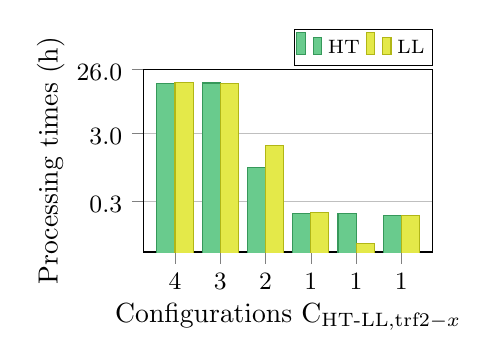
\begin{tikzpicture}[text depth=0pt]
\begin{axis}[width=5.25cm,
height=3.9cm,
log basis y={10},
ymajorgrids,
tick align=outside,
tick pos=left,
xlabel={Configurations C$_{\text{HT-LL,trf2}-x}$},
xmin=-0.69, xmax=5.69,
xtick={0,1,2,3,4,5},
xticklabels={4,3,2,1,1,1},
ylabel={Processing times (h)},
ymin=197.09433652085, ymax=78839.0699338796,
ymode=log,
ytick={1080,10800,93600},
ymax=93600,
yticklabels={0.3,3.0,26.0},
xticklabel style={yshift=2pt},
xlabel style={yshift=2pt},
legend cell align={left},
legend columns=-1,
legend style={
	font=\scriptsize,
	fill opacity=1,
	draw opacity=1,
	text opacity=1,
	at={(1.0,1.02)},
	anchor=south east,
	inner sep=0.75pt,
},
colormap/viridis,
%xlabel style={font=\Large},
%ylabel style={font=\Large},
xticklabel style={font=\small},
yticklabel style={font=\small},
typeset ticklabels with strut, 
]
\draw[bar-color=700] (axis cs:-0.4,0) rectangle (axis cs:0,58524.9786317348);
\addlegendimage{ybar,ybar legend,bar-color=700};
\addlegendentry{HT}

\draw[bar-color=700] (axis cs:0.6,0) rectangle (axis cs:1,59219.2741601467);
\draw[bar-color=700] (axis cs:1.6,0) rectangle (axis cs:2,3407.09036183357);
\draw[bar-color=700] (axis cs:2.6,0) rectangle (axis cs:3,719.325023651123);
\draw[bar-color=700] (axis cs:3.6,0) rectangle (axis cs:4,712.563487291336);
\draw[bar-color=700] (axis cs:4.6,0) rectangle (axis cs:5,677.699569702148);
\draw[bar-color=950] (axis cs:-2.77555756156289e-17,0) rectangle (axis cs:0.4,60043.459069252);
\addlegendimage{ybar,ybar legend,bar-color=950};
\addlegendentry{LL}

\draw[bar-color=950] (axis cs:1,0) rectangle (axis cs:1.4,59003.3924343586);
\draw[bar-color=950] (axis cs:2,0) rectangle (axis cs:2.4,7238.57805323601);
\draw[bar-color=950] (axis cs:3,0) rectangle (axis cs:3.4,737.270066261292);
\draw[bar-color=950] (axis cs:4,0) rectangle (axis cs:4.4,258.791455745697);
\draw[bar-color=950] (axis cs:5,0) rectangle (axis cs:5.4,675.399163722992);
\end{axis}
\end{tikzpicture}
\end{document}